\documentclass[../main.tex]{subfiles}
\graphicspath{{\subfix{../images/}}}
\begin{document}
\section*{Term 2 Week 6}
\begin{enumerate}
    \item 
    There are 4 squares, each with area of 16cm\(^2\), inside a circle as shown below. Calculate the \textbf{exact} area of the circle.
    \begin{figure}[h]
        \centering
        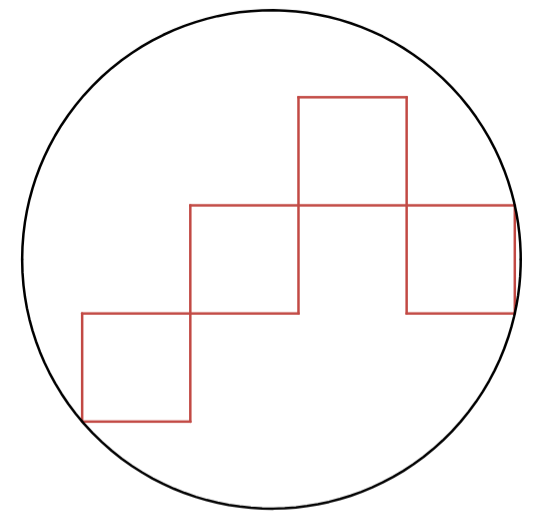
\includegraphics[width=0.3\linewidth]{images/t2w6q1.png}
    \end{figure}
    
    \item 
    If \(a^2+b^2+c^2+d^2=4\)\\
    Where \(a,b,c,d \in \mathbb{R}\):
        \begin{enumerate}
            \item 
            Show that \((a+2)(b+2)\geq cd\)\\

            \item 
            Determine when \((a+2)(b+2)=cd\)\\
        \end{enumerate}

    \item 
    Solve for \textbf{x}:\\

    \(\log_{\log_3{x}}{9}=\log_3{(\log_{27}{x})}\)\\

    \item 
    In triangle \textit{ABC}, the altitude (h) from \textit{A} divides the side \textit{BC} into segments of length 3 and 17.\\
    Given that \(\tan{(\angle CAB)}=\frac{22}{7}\), find the \textbf{exact} area of triangle \textit{ABC}.
    \begin{figure}[h]
        \centering
        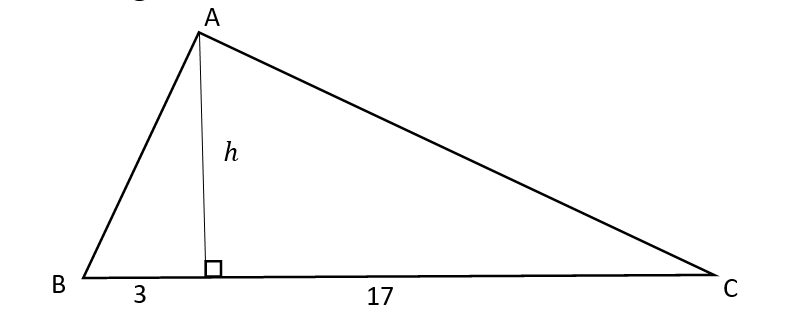
\includegraphics{images/t2w6q4.png}
    \end{figure}
    
    \end{enumerate}

\end{document}